% siminos/CLE/symSol.tex
% $Author$ $Date$

\section{\label{s:symSol} Symmetries of solutions}

A complete classification of solutions in systems with
continuous symmetries is beyond the scope of this paper. Here
we concentrate on particular types of solutions that play an
important dynamical role in the examples we will consider and
also help explain the need for symmetry reduction.

The \emph{group orbit} or $\Group$-orbit of
$x\in\Rls{n}$ is the set
\beq
	\Group x = \{\LieEl x: \LieEl\in\Group\}\,
\eeq
of all points in which $x$ is mapped under the action of all
group elements of $\Group$.
A set of group actions which maps a \statesp\ point $\ssp$ into itself,
\beq
\stab{\ssp} =\{\LieEl \in \Group: \LieEl \ssp = \ssp \}
    \,,
\ee{def:isotr}
is called the \emph{isotropy} (or \emph{stabilizer})  group of $\ssp$.
The isotropy subgroup is the largest subgroup (in the
sense of set inclusion) that leaves $\ssp$ fixed.
The \emph{group of symmetries} of a set $X$ is the largest
subgroup $\Subgroup_X$ that leaves $X$ invariant as a set:
\beq
	\Group_X= {\LieEl: \LieEl X = X}\,.
\eeq

The \emph{\fixedsp} of any subgroup $\Subgroup\subset\Group$,
denoted by $\Fix{\Subgroup}$, is the subspace of $\Manif$ containing all fixed points of $\Sigma$:
\[
	\Fix{\Sigma}=\{\ssp\in\Manif\ |\ \sigma \ssp = \ssp\,,\ \forall \sigma\in\Sigma\}\,.
\]

\Fixedsp s are invariant under $\Group$-equivariant dynamics\rf{golubitsky2002sp},
\[
 f^t\left(\Fix{\Subgroup}\right)\subseteq \Fix{\Subgroup}
\] for all
$t$. Therefore if $\ssp(t)$ is a solution trajectory of an
equivariant ODE then $\stab{\ssp(t)}=\stab{\ssp(0)}$ for all $t$.


In contrast to \emph{\eqv} solutions that satisfy
$f^\tau(\ssp) - \ssp = 0$, \emph{\reqva} satisfy
$f^\tau(\ssp) - \LieEl( \tau) \, \ssp= 0$ for any $\tau$. In
a co-moving frame, \ie, a frame moving along the group orbit
with velocity $\vel(\ssp) = \velRel \cdot \groupTan(\ssp)$,
    \ES{define $\groupTan$ in symmetry section, choose
    a prettier symbol. {\bf PC:} I see it coming; you will
    make it all look Greek to me. {\bf ES:} Well, unless
	you want to change time to $\tau$ we have to change
	group tangent. {\bf PC:} I do call time $\tau$ in
    continuous.tex .}
the \reqv\ appears as an \eqv.

A {\em \rpo} $p$ is an orbit $\pS_p$ in {\statesp} $\pS$
which exactly recurs
    \index{periodic!orbit!relative}\index{relative!periodic orbit}
\beq
\ssp_p (0) = \LieEl_p \ssp_p (\period{p} )
    \,,\qquad
\ssp_p (\tau) \in \pS_p
    \,,
\label{RPOrelper1}
\eeq
at a fixed {\em relative period} $\period{p}$, but
shifted by a fixed group action ${\LieEl_p}$
which brings the endpoint $\ssp_p (\period{p} ) $
back into the initial point $\ssp_p (0) $, see \reffig{f:rpo}.
The group action ${\LieEl_p}$ parameters
$\gSpace = (\gSpace_1,\gSpace_2,\cdots\gSpace_N)$
will be referred to as ``phases,'' or ``shifts.''
% In contrast to the pre-periodic \refeq{preperiodic},
The phases here are irrational, and the trajectory sweeps out
ergodically the group orbit without ever closing into a \po.
For dynamical systems with only continuous (no discrete)
symmetries, the parameters $\{t,\gSpace_1,\cdots,\gSpace_N\}$
are real numbers, ratios $\pi/\gSpace_j$ are almost never
rational, the likelihood of finding a {\po} for such system is
{zero}, and such \rpo s are almost never eventually periodic.

%
%%%%%%%%%%%%%%%%%%%%%%%%%%%%%%%%%%%%%%%%%%%%%%%%%%%%%%%%%%%%%%%%
% hand-drawn in dasbuch/book/FigSrc/xfig/rpo.fig
\begin{figure}[ht]
(a)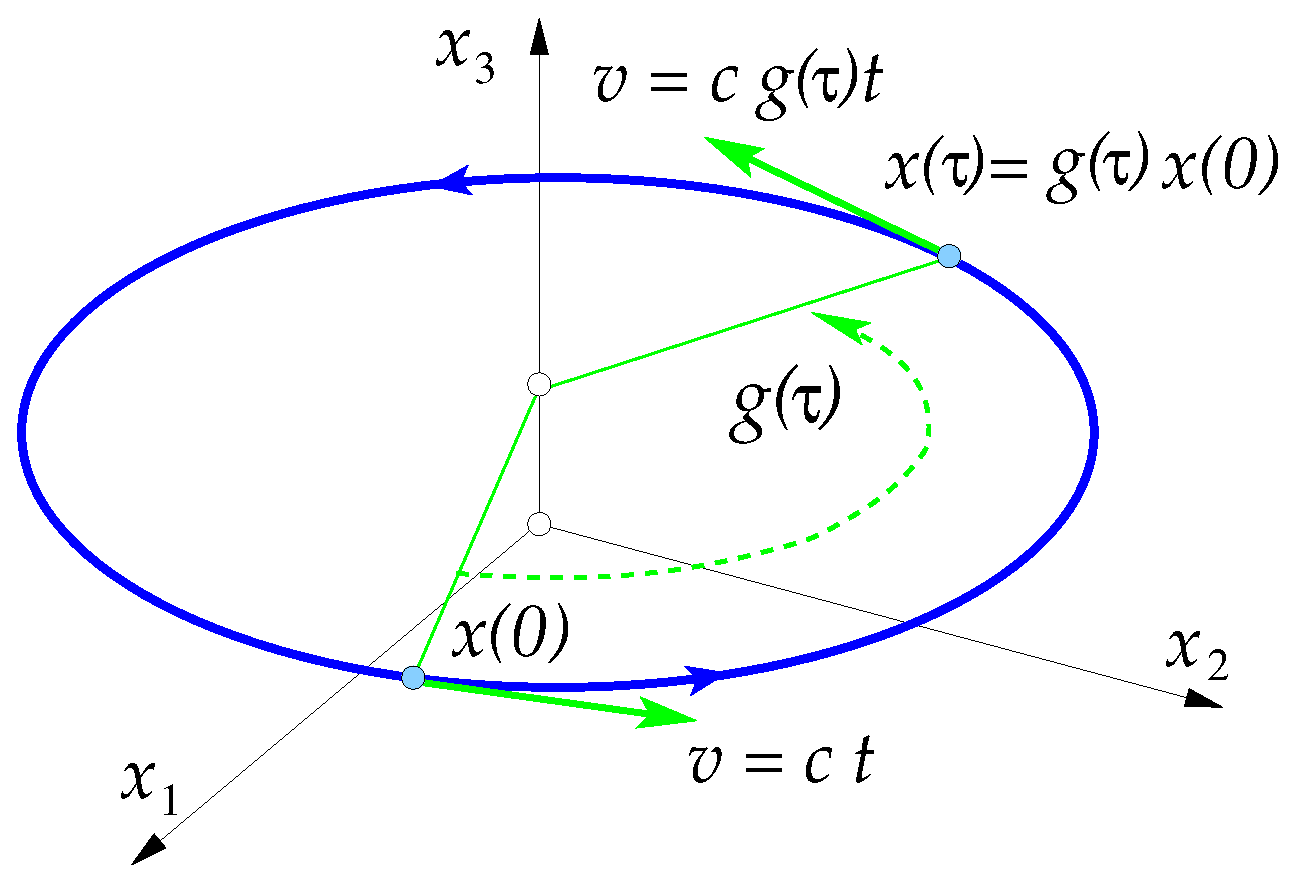
\includegraphics[width=0.3\textwidth]{../Fig/reqv.eps}
(b)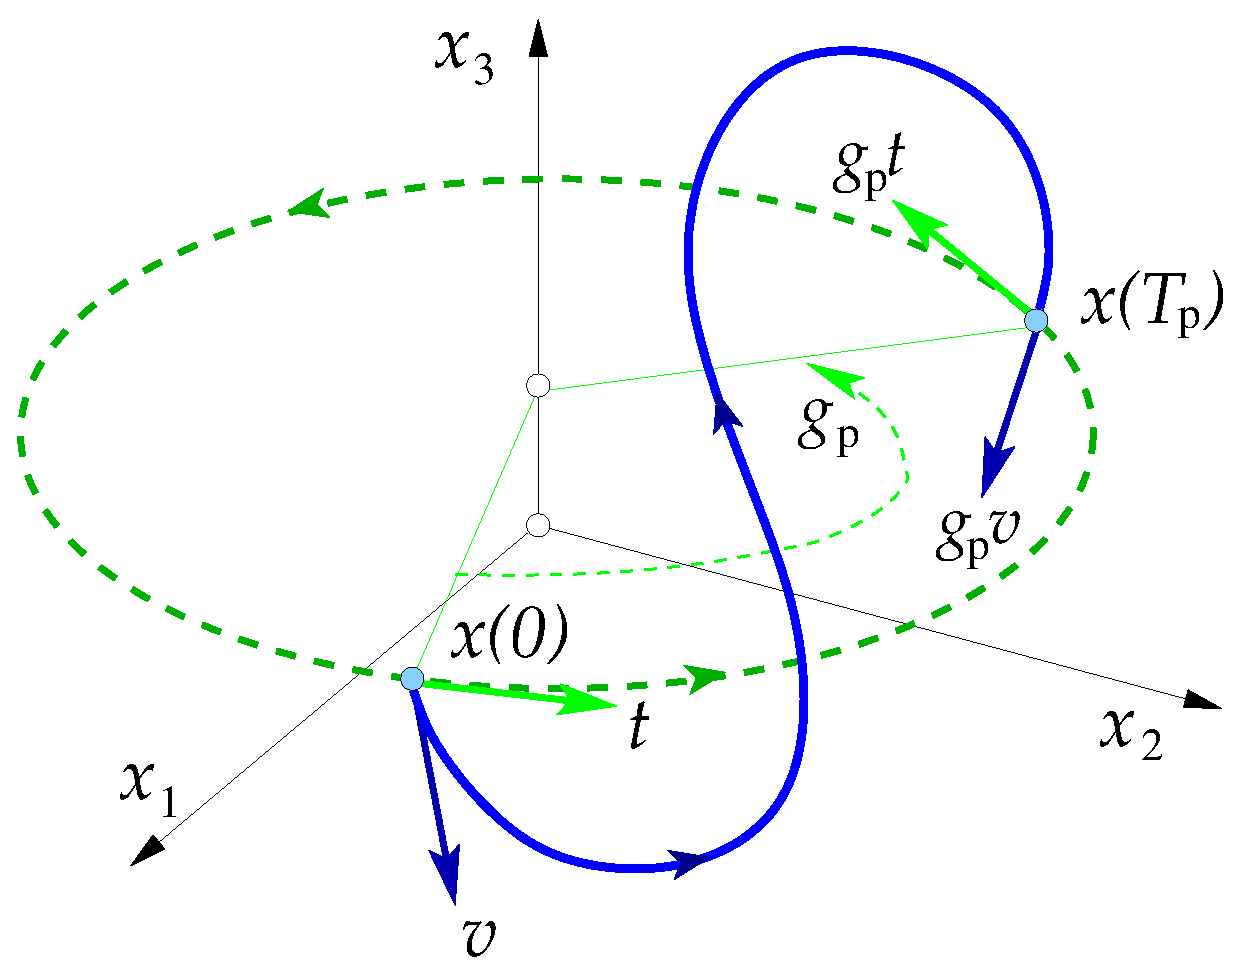
\includegraphics[width=0.3\textwidth]{../Fig/rpo.eps}
\caption{
(a) A {\em \reqv\ orbit} starts out at some point $\ssp(0)$,
with the dynamical flow field $\vel(\ssp) = \velRel \cdot
\groupTan(\ssp)$ pointing along the group tangent space. For
the $\SOn{2}$ symmetry depicted here, the flow traces out the
group orbit of $\ssp(0)$ in time $\period{}=2\pi/\velRel$.
An
{\em \eqv} lives either in the fixed $\Fix{\Group}$ subspace
($x_3$ axis in this sketch), or on a group orbit as the one
depicted here, but with zero angular velocity $\velRel$. In
that case the circle (in general, $N$-torus) depicts a
continuous family of fixed \eqva, related only by the group
action.
(b) A \rpo\ starts out at $\ssp(0)$ with the dynamical $\vel$ and
group tangent $\groupTan$ flows pointing in different
directions, and returns to the group orbit of $\ssp(0)$ after
time $\period{p}$ at $\ssp(\period{p})=\LieEl_p \ssp (0)$, a
rotation of the initial point by $\LieEl_p$.
}
\label{f:rpo}
\end{figure}
%%%%%%%%%%%%%%%%%%%%%%%%%%%%%%%%%%%%%%%%%%%%%%%%%%%%%%%%%%%%%%%%%%

Similarly to a \reqv, a \emph{\rpo} is periodic in its
mean velocity $\velRel_p=\gSpace_p/\period{p}$ co-rotating
frame (see \reffig{f:MeanVelocityFrame}), but in the
stationary frame its trajectory is quasiperiodic.
A co-moving
frame is helpful in visualizing a single `relative' orbit,
but useless for viewing collections of orbits, as each one
drifts with its own angular velocity. Visualization of all
\rpo s as \po s we attain only by global\marginpar{explain global vs
local in intro. It is not really global.} symmetry reduction,
to be undertaken in the following.

%
%%%%%%%%%%%%%%%%%%%%%%%%%%%%%%%%%%%%%%%%%%%%%%%%%%%%%%%%%%%%%%%%
% from siminos/rpo_ks/arxiv-v2/figs
\begin{figure}[ht]
(a)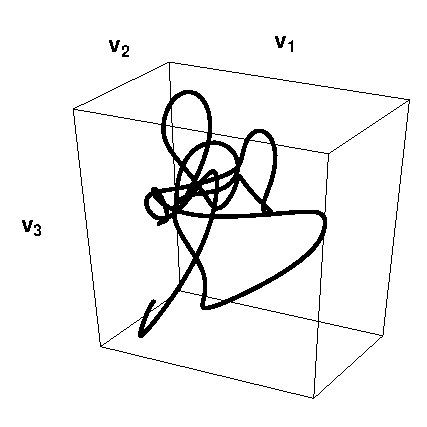
\includegraphics[width=0.37\textwidth, clip=true]
                    {../figs/ks22rpo033.50_04.045E2.eps}
~(b)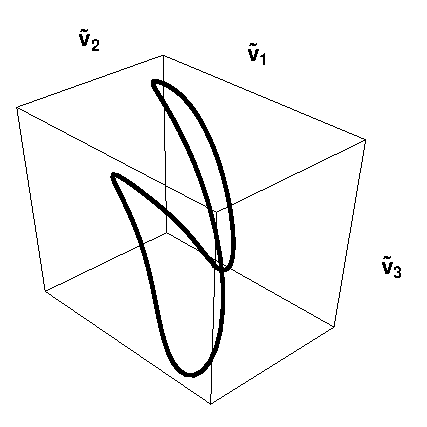
\includegraphics[width=0.37\textwidth, clip=true]
                     {../figs/ks22rpo033.50_04.045E2CM.eps}
\caption{
 A \rpo\ of Kuramoto-Sivashinsky flow projected on
 (a) the stationary \statesp\ coordinate frame
 $\{v_1,v_2,v_3\}$, traced for four periods
 $\period{p}$;
 (b) the co-moving $\{\tilde{v}_1,\tilde{v}_2,\tilde{v}_3\}$
 coordinate frame, moving with the mean angular velocity
 $\velRel_p=\gSpace_p/\period{p}$.
\hfill (from \refref{SCD07})
}
\label{f:MeanVelocityFrame}
\end{figure}
%%%%%%%%%%%%%%%%%%%%%%%%%%%%%%%%%%%%%%%%%%%%%%%%%%%%%%%%%%%%%%%%%%
